\section{Related works}

\subsection{Notations}

\subsubsection{Continuous Time domain}
\begin{align}
  \mathbb{T} = [0, 1]
\end{align}

\subsubsection{Discrete Time domain}
\begin{align}
  \mathcal{T} = \left\{t_1 = t_\epsilon = \epsilon, t_2, \cdots, t_N = T = 1\right\}
\end{align}

\subsubsection{Discrete trajectory}
\begin{align}
  \left\{ \mathbf{x}_t \right\}_{t \in \mathcal{T}}
\end{align}

\noindent With $\mathbf{x}_{\epsilon} \approx \mathbf{x}_0$ is the fully denoised image, and $\mathbf{x}_T \sim \mathcal{N}(0, I)$ is the initial condition (fully noised image). \\

\subsection{Discrete ODE solver}
\begin{align}
    \widehat{\mathbf{x}}_{t_n}^{\phi} &= \mathbf{x}_{t_{n+1}} + (t_n  -t_{n+1}) \Phi(\mathbf{x}_{t_{n+1}}, t_{n+1}; \phi)
\end{align}
\noindent With $\Phi(\mathbf{x}_{t_{n+1}}, t_{n+1}; \phi)$ a score function.

\subsection{Consistency Models}
\noindent Consistency Models (\cite{song2023consistencymodels}) learn a function $f_{\theta}$ that maps any point of the trajectory $\mathbf{x}_t $ to the last point of the trajectory $\mathbf{x}_{\epsilon}$:

\begin{align}
  f_{\theta}(\mathbf{x}_t, t) &= \widehat{\mathbf{x}}_{\epsilon} \;, \; \forall t \in \mathcal{T} \setminus \epsilon \\
  f_{\theta}(\mathbf{x}_{\epsilon}, t) &= \mathbf{x}_{\epsilon} \: \: \text{(Boundary Condition)}
\end{align}

\subsection{Continuous Time Consistency Models}
\noindent In \cite{lu2025simplifyingstabilizingscalingcontinuoustime}, authors extend Consistency Models by using Continuous Time formulation ($t \in \mathbb{T}$). They also introduce the TrigFlow parametrization that stabilizes training and allow the model to scale:
\begin{align}
    \frac{d\mathbf{x}_t}{dt} &= \cos(t)\, f_\theta(x, t) - \sin(t)\, \nabla_{\mathbf{x}} f_\theta(\mathbf{x}, t).
\end{align}

\noindent They ensure velocity consistency:
\begin{align}
    \frac{d\:f_{\theta}(\mathbf{x}_t, t)}{dt} = 0
\end{align}

\subsection{Neural Operators}
\noindent \cite{zheng2023fastsamplingdiffusionmodels} learns an operator $\mathcal{G}_{\theta}^{T}$ that, for a given initial condition $\mathbf{x}_T$, forecasts the entire trajectory:

\begin{align}
   \mathcal{G}_{\theta}^{T}(\mathbf{x}_T, T) = \left\{\widehat{\mathbf{x}}_t\right\}_{\forall t \in \mathcal{T}}
\end{align}

\noindent Note that other papers in the Neural Operator field \cite{ganeshram2025fcpinohighprecisionphysicsinformed} rarely deal with image generation, but focus on PDE solving in several dimension. 

\subsection{Flow Map Matching}
\noindent \cite{boffi2025flowmapmatchingstochastic} formalize the flow match mapping as:
\begin{align}
    X_{t, s} \: \: : \mathbf{x}_t & \mapsto \mathbf{x}_s, \: (s, t) \in \mathbb{T}^2 \\
    X_{t, \tau}(X_{s, t}(x)) & = X_{s, \tau} \: \: \text{consistency property}
\end{align}

\subsection{Flow Matching with Consistent Velocity}
\noindent \cite{yang2024consistencyflowmatchingdefining} Consider the velocity $v$ of a flow $\mathbf{X}$ ($t \in \mathbb{T}$):
\begin{align}
    v_{\theta}(\mathbf{x}_t, t) &= \frac{d \mathbf{X}_{T, t}}{dt} \\
    f_{\theta}(\mathbf{x}_t, t) & = \mathbf{x}_t + t * v_{\theta}(\mathbf{x}_t, t) = \widehat{\mathbf{x}}_{\epsilon}
\end{align}

\noindent They then enforce Velocity Consistency :
\begin{align}
    v_{\theta}(\mathbf{x}_t, t) = v_{\theta}(\mathbf{x}_T, T)
\end{align}

\subsection{Summary}
\noindent A summary of the different categories of methods from the literature is shown in Figure~\ref{fig:models}

\begin{figure}[htbp]
  \centering
  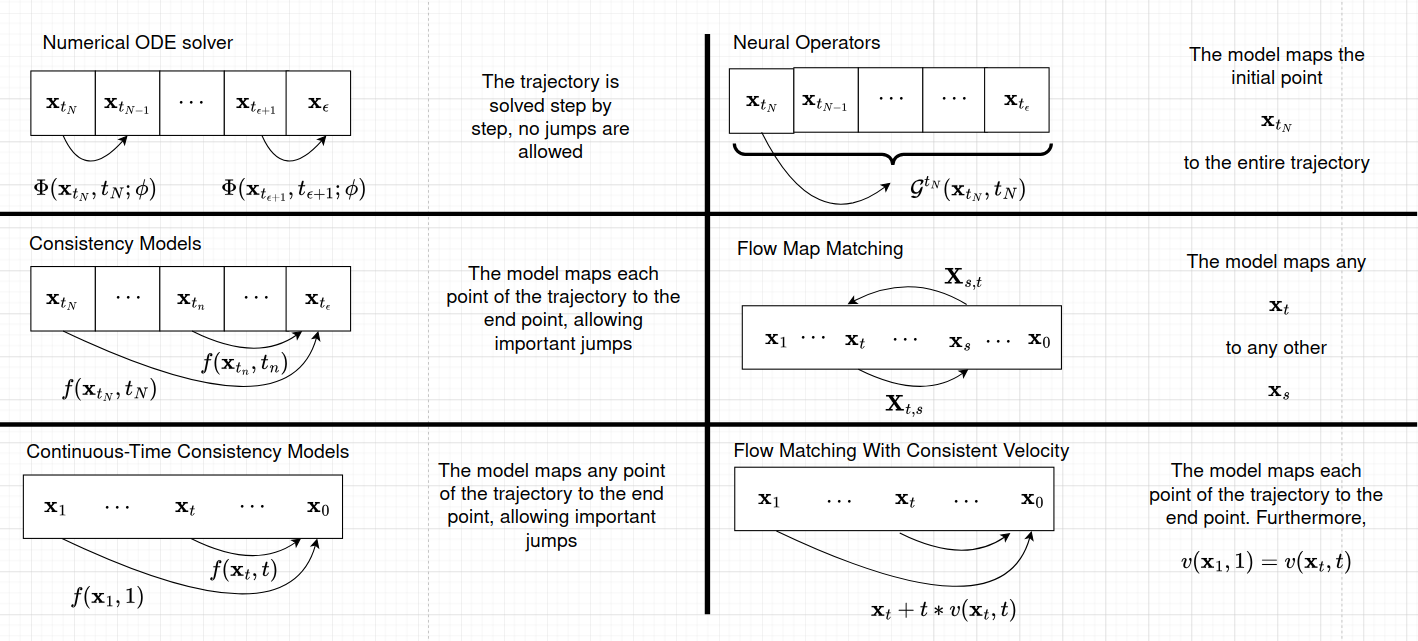
\includegraphics[width=1.2\textwidth]{figures/models.png}
  \caption{A visual summary of the different approaches for image generation from noise.}
  \label{fig:models}
\end{figure}